\chapter{Confronting the MSSM with the muon $(g-2)_{\mu}$ and dark matter}
\label{chap:muong-2}

\chapterquote{I have done a terrible thing, I have postulated a particle that cannot be detected.}
{Wolfgang Pauli, 1900--1958}

\section{Implications for low-energy observables}
\label{sec:MSSMconstraints}

Many constraints on the MSSM that are relevant come from low-energy observables. In section \ref{subsec:MSSMsoftbreak}, we discussed how constraints from flavour-changing and $CP$-violating effects typically result in certain structure for the scalar mass matrices. However, this is not all. There are also constraints coming from astrophysical observations, where one of these is from the MSSM neutralino as an explanation for the observed dark matter.

We will discuss the relevant sources of constraint in detail below since our phenomenological studies will be confronted with them.

\begin{enumerate}
\item \textbf{LHC, LEP and Tevatron constraints.} The most straightforward constraint imposed on the SUSY spectrum should be that the lightest Higgs boson mass should be SM-like. Recently, the \acrshort{atlas} and \acrshort{cms} collaborations at \acrshort{lhc} have discovered a new boson that resembles a Standard Model Higgs boson with a mass of roughly 125 GeV \cite{RN62,RN63}. When considering the Higgs boson mass in SUSY, we should include radiative corrections, with the main contribution from the stop squark at one-loop in Eq. \ref{eqn:higgsmass}. In addition, since the Higgs sector in the MSSM is extended compared to the SM, it should be confronted with precision measurements. The main processes at \acrshort{lep} (Large Electron-Positron Collider) come from Higgsstrahlung and double Higgs production, whilst Tevatron limits come from gluon fusion, Higgsstrahlung, VBF and associated production processes.

One can typically avoid constraints on the SM-like Higgs boson in the so-called '\textit{decoupling limit}' \cite{RN572}. Typically any theory containing a light Higgs boson of mass $m_h$ and a number of heavier Higgses of mass $M$ will have its effects suppressed by the ratio $m^2_{h}/M^2$, since operators in the effective Lagrangian describing perturbations to the Higgs coupling will enter with dimension 6. This is particularly characteristic of the MSSM Higgs sector since the heavier Higgs particles all appear on the order of the pseudoscalar mass $m_{A^0}$ whilst the lighter Higgs boson is $\sim m_Z$ at tree-level. Hence, with heavier contributions at the TeV scale, the corrections to the lighter Higgs couplings are already reduced to around a percent level.

Direct searches have also been performed for the first two generations of sleptons and the lightest chargino. LEP has produced the following limits \cite{RN493}:
\begin{eqnarray}
m_{\tilde{\ell}_L},m_{\tilde{\ell}_R} &>& 100\,\text{GeV}, \qquad (\ell=e,\mu), \\
m_{\tilde{\chi}^{\pm}_1} &>& 105\,\text{GeV}.
\end{eqnarray}

\item \textbf{Flavour and $CP$-violating constraints.}

Flavour mixing in the MSSM can be induced in both the squark and slepton sectors, leading to particularly dangerous sources of flavour-violating processes, which experiments suggest are strongly suppressed.

\begin{enumerate*}
\setlength\itemsep{1em}

\item[] \textbf{$\mu \rightarrow e\gamma$}
\newline

The process $\mu \rightarrow e\gamma$ can be induced through slepton-neutralino or sneutrino-chargino loops. This depends on the off-diagonal contributions from $m^2_{\bar{e}}$, $m^2_{\tilde{Q}}$ or $A_{e}$.
\begin{center}
\scalebox{0.65}{
\fcolorbox{white}{white}{
  \begin{picture}(354,136) (159,-91)
    \SetWidth{1.0}
    \SetColor{Black}
  \Line[arrow,arrowpos=0.5,arrowlength=5,arrowwidth=2,arrowinset=0.2](160,-88)(256,-88)
  \Arc[dash,dashsize=10,arrow,arrowpos=0.25,arrowlength=5,arrowwidth=2,arrowinset=0.2,clock](336,-88)(80,-180,-360)
  \Arc[dash,dashsize=10,arrow,arrowpos=0.75,arrowlength=5,arrowwidth=2,arrowinset=0.2,clock](336,-88)(80,-180,-360)
  \Line[arrow,arrowpos=0.5,arrowlength=5,arrowwidth=2,arrowinset=0.2](416,-88)(512,-88)
  \Line[arrow,arrowpos=0.5,arrowlength=5,arrowwidth=2,arrowinset=0.2](256,-88)(416,-88)
  \Line(331,-3)(341,-13)\Line(331,-13)(341,-3)
    \Photon(394,-30)(442,18){7.5}{3}
    \Text(448,24)[lb]{\Large{\Black{$\gamma$}}}
    \Text(208,-75)[lb]{\Large{\Black{$\mu$}}}
    \Text(464,-75)[lb]{\Large{\Black{$e$}}}
    \Text(270,-15)[lb]{\Large{\Black{$\tilde{\mu}_L$}}}
    \Text(380,-15)[lb]{\Large{\Black{$\tilde{e}_L$}}}
    \Text(332,-75)[lb]{\Large{\Black{$\tilde{\chi}^0$}}}
    \Text(312,8)[lb]{\Large{\Black{$(\delta^{LL}_{\tilde{L}})_{12}$}}}
  \end{picture}
}}
\vspace{5mm}
\captionof{figure}[MSSM contribution to the lepton flavour-changing process $\mu \rightarrow e\gamma$.]{A supersymmetric contribution to the lepton flavour-changing process $\mu \rightarrow e\gamma$ coming from off-diagonal terms in the slepton mass-squared matrix $m^2_{\bar{e}}$. Current upper limit on the branching fraction is $\mathcal{B}(\mu \rightarrow e\gamma)<2.4\times 10^{-12}$ \cite{RN571}.}
\label{fig:muegamma}
\end{center}

In the mass insertion approximation \cite{RN574,RN669}, we describe the off-diagonal terms ($i\neq j$) in the slepton mass matrix (flavour space) with
\begin{equation}
(\delta^{LL}_{\tilde{L}})_{ij}=\frac{(\Delta m_{\tilde{L}}^2)_{ij}}{m_{\tilde{L}}^2},
\end{equation}
where $m_{\tilde{L}}^2$ is the average slepton mass squared. The off-diagonal mixing terms are treated as a perturbation to the slepton mass term. Then the branching fraction of muon decay to $e\gamma$ relative to $\mathcal{B}(\mu \rightarrow e\nu_{\mu}\overline{\nu}_{e})$ is \cite{RN575}:
\begin{equation}
\mathcal{B}(\mu \rightarrow e\gamma) \sim 10^{-5}\left(\frac{m_W}{M_{SUSY}}\right)^4|(\delta^{LL}_{\tilde{L}})_{12}|^2 \tan^2\beta.
\end{equation}
For an $M_{SUSY}$ of around 1 TeV, one can reduce the ratio to about $10^{-8}-10^{-9}$ assuming an insertion parameter of order unity. The current experimental bound is $\mathcal{B}(\mu \rightarrow e\gamma)<2.4\times 10^{-12}$ \cite{RN571}. Hence, we would expect quite a suppression in the off-diagonal terms in the slepton mass matrix compared to the diagonal (non-flavour violating) components.

\item[] \textbf{$K^{0}\overline{K}^{0}$-mixing}
\newline

Similarly, there is constraint on the squark mass-squared matrices coming from neutral kaon mixing. Some of these can be important especially the squark-quark-gluino vertex, shown in Figure \ref{fig:KKmixing} which are of the order of $\alpha^2_S$ where $\alpha_S=g^2_S/4\pi$ is the strong analogue of the fine-structure constant. Clearly diagrams of this type only become valid in the limit of non-zero down-squark mass mixing, shown by the mass insertions $(\delta^{LL}_{\tilde{Q}})_{12}$, $(\delta^{RR}_{\bar{d}})_{12}$ and $(\delta^{LR}_{\bar{d}})_{12}$ depending on whether the mixing (off-diagonal terms) come from the soft-SUSY breaking matrices $m^2_{\tilde{Q}}$, $m^2_{\bar{d}}$ or $A_d$. Here, the mixing terms are again treated as a perturbation to nearly degenerate squark masses.
\begin{center}
\scalebox{0.65}{
\fcolorbox{white}{white}{
  \begin{picture}(308,166) (271,-139)
    \SetWidth{1.0}
    \SetColor{Black}
\Line[arrow,arrowpos=0.5,arrowlength=5,arrowwidth=2,arrowinset=0.2](272,-122)(352,-122)
\Line[arrow,arrowpos=0.5,arrowlength=5,arrowwidth=2,arrowinset=0.2](352,-10)(272,-10)
\Line(352,-10)(352,-122)
\Line[dash,dashsize=10](352,-10)(464,-10)
\Line[dash,dashsize=10](352,-122)(464,-122)
\Line[arrow,arrowpos=0.5,arrowlength=5,arrowwidth=2,arrowinset=0.2](544,-10)(464,-10)
\Line[arrow,arrowpos=0.5,arrowlength=5,arrowwidth=2,arrowinset=0.2](464,-122)(544,-122)
\Line(464,-10)(464,-122)
    \Line(403,-15)(413,-5)\Line(403,-5)(413,-15)
    \Line(403,-127)(413,-115)\Line(403,-115)(413,-127)
    \Text(334,-74)[lb]{\Large{\Black{$\tilde{g}$}}}
    \Text(476,-74)[lb]{\Large{\Black{$\tilde{g}$}}}
    \Text(274,0)[lb]{\Large{\Black{$\overline{s}$}}}
    \Text(274,-112)[lb]{\Large{\Black{$d$}}}
    \Text(540,0)[lb]{\Large{\Black{$\overline{d}$}}}
    \Text(540,-112)[lb]{\Large{\Black{$s$}}}
    \Text(368,0)[lb]{\Large{\Black{$\tilde{s}^{*}_R$}}}
    \Text(368,-112)[lb]{\Large{\Black{$\tilde{d}_R$}}}
    \Text(442,0)[lb]{\Large{\Black{$\tilde{d}^{*}_R$}}}
    \Text(442,-112)[lb]{\Large{\Black{$\tilde{s}_R$}}}
    \Text(388,-45)[lb]{\Large{\Black{$(\delta^{RR}_{\bar{d}})_{12}$}}}
    \Text(388,-157)[lb]{\Large{\Black{$(\delta^{RR}_{\bar{d}})_{12}$}}}
  \end{picture}
}}
\vspace{5mm}
\captionof{figure}[MSSM contribution to $K^{0}\overline{K}^{0}$ mixing.]{A contribution from supersymmetry to $K^{0}\overline{K}^{0}$ mixing through gluino-squark loops. In the mass insertion approximation, the vertices (represented by $\times$) are the off-diagonal elements of $m^2_{\bar{d}}$. One can also have contributions from $(\Delta m^2_{\tilde{Q}})_{12}$, a combination of $(\Delta m^2_{\tilde{Q}})_{12}$ and $(\Delta m^2_{\bar{d}})_{12}$ or $(\Delta A_d)_{12}$ depending on the quark helicity states.}
\label{fig:KKmixing}
\end{center}
Generically, one can calculate the contributions from the effective Hamiltonian $\mathcal{H}^{\Delta S=2}_{\text{eff}}$ \cite{RN670,RN673,RN674},
\begin{equation}
\mathcal{H}^{\Delta S=2}_{\text{eff}}=\sum_{i=1}^{5}C_{i}\mathcal{O}_{i}+\sum_{i=1}^{3}\tilde{C}_{i}\tilde{\mathcal{O}}_{i},
\end{equation}
where the operators $\mathcal{O}_i$ and $\tilde{\mathcal{O}}_i$ are defined to be:
\begin{alignat}{2}
\mathcal{O}_{1}&=(\overline{s}^{i}_{L}\gamma^{\mu}d^{i}_{L})(\overline{s}^{j}_{L}\gamma_{\mu}d^{j}_{L}),& \quad \tilde{\mathcal{O}}_{1}&=\mathcal{O}_{1}(L \leftrightarrow R), \\
\mathcal{O}_{2}&=(\overline{s}^{i}_{R}d^{i}_{L})(\overline{s}^{j}_{R}d^{j}_{L}),& \quad \tilde{\mathcal{O}}_{2}&=\mathcal{O}_{2}(L \leftrightarrow R), \\
\mathcal{O}_{3}&=(\overline{s}^{i}_{R}d^{j}_{L})(\overline{s}^{j}_{R}d^{i}_{L}),& \quad \tilde{\mathcal{O}}_{3}&=\mathcal{O}_{2}(L \leftrightarrow R), \\
\mathcal{O}_{4}&=(\overline{s}^{i}_{L}d^{i}_{R})(\overline{s}^{j}_{R}d^{j}_{L}),& \quad \tilde{\mathcal{O}}_{5}&=(\overline{s}^{i}_{L}d^{j}_{R})(\overline{s}^{j}_{R}d^{i}_{L}). 
\end{alignat}
After matching effective Hamiltonian with the full theory one can compute the Wilson coefficients $C_i$ and $\tilde{C}_i$, and hence the observables
\begin{eqnarray}
&&\Delta m_{K}=2 \text{Re}\left[ \bra{K^{0}} \mathcal{H}^{\Delta S=2}_{eff} \ket{\overline{K}^{0}} \right] \label{eqn:mK},\\
&&\epsilon_{K}=\frac{1}{\sqrt{2}\Delta m_{K}}\text{Im}\left[ \bra{K^{0}} \mathcal{H}^{\Delta S=2}_{eff} \ket{\overline{K}^{0}} \right]. \label{eqn:epsilonK}
\end{eqnarray}
where Eqs. \ref{eqn:mK} and \ref{eqn:epsilonK} are the $\Delta m_K \equiv m_{K_{L}}-m_{K_{S}}$ mass eigenstate difference and $\epsilon_{K}$ is the $CP$-violating parameter. Constraints on the experimentally measured values can be interpreted in terms of the real and imaginary parts of the mass insertion parameters and the ratio of the gluino to the average squark mass, $m^2_{\tilde{g}}/m^2_{\tilde{q}}$ \cite{RN670}. Similar, but weaker, constraints come from other systems like $D^{0}\overline{D}^{0}$ mixing which puts constraints on the amount of sup-scharm mixing, for example.

\end{enumerate*}

\item \textbf{$B$-Physics observables}

In SUSY, the flavour structure of the soft breaking terms can contribute to processes involving $B$ and $K$ mesons. We discuss the most relevant of these to this thesis in this section.

\begin{enumerate*}
\setlength\itemsep{1em}

\item[] \textbf{$b \rightarrow s\gamma$}
\newline

The FCNC decay $b \rightarrow s\gamma$ is highly sensitive to new physics, and thus has sizable contributions from SUSY. At lowest order, the decay proceeds in the SM through a $tW$ loop, however SUSY contributions contain an additional charged Higgs and other coloured sparticle loops. One can write the new physics contributions to $b \rightarrow s\gamma$ with the effective Hamiltonian, where particles above the scale $Q=m_W$ are integrated out \cite{RN576},
\begin{equation}
\mathcal{H}^{\Delta F=1}_{\text{eff}}	=-\frac{4G_{F}}{\sqrt{2}}V^{*}_{ts}V_{tb}\sum^{8}_{i=1}C_{i}(Q)\mathcal{O}_{i}, 
\end{equation}
The new physics contributions can appear dominantly through the magnetic and chromomagnetic operators, given in \cite{RN672} as:
\begin{align}
\mathcal{O}_{7}&=\frac{e}{16\pi^2}m_{b}(\overline{s}\sigma^{\mu\nu}P_{R}b)F_{\mu\nu}, \\
\mathcal{O}_{8}&=\frac{g_{s}}{16\pi^2}m_{b}(\overline{s}\sigma^{\mu\nu}T^{a}P_{R}b)G^{a}_{\mu\nu}.
\end{align}
New physics contributions from SUSY at one-loop to the Wilson coefficients are found by matching to the full theory at $Q=m_W$ and are given as
\begin{equation}
C^{SUSY}_{7,8}=C^{H^{\pm}}_{7,8}+C^{\tilde{\chi}^{\pm}}_{7,8}+C^{\tilde{g}}_{7,8}+C^{\tilde{\chi}^0}_{7,8},
\end{equation}
which are penguin diagrams containing charged Higgs-up type quarks, charginos-up type quarks, gluino-down type quarks and neutralino-down type quarks respectively.
\begin{center}
\scalebox{0.65}{
\fcolorbox{white}{white}{
  \begin{picture}(612,150) (143,-123)
    \SetWidth{1.0}
    \SetColor{Black}
    \Line[arrow,arrowpos=0.5,arrowlength=5,arrowwidth=2,arrowinset=0.2](144,-106)(208,-106)
    \Line[arrow,arrowpos=0.5,arrowlength=5,arrowwidth=2,arrowinset=0.2](336,-106)(400,-106)
    \Line[arrow,arrowpos=0.5,arrowlength=5,arrowwidth=2,arrowinset=0.2](480,-106)(544,-106)    \Arc[arrow,arrowpos=0.25,arrowlength=5,arrowwidth=2,arrowinset=0.2,clock](272,-106)(64,-180,-360)
 \Arc[arrow,arrowpos=0.75,arrowlength=5,arrowwidth=2,arrowinset=0.2,clock](272,-106)(64,-180,-360)
 \Arc[dash,dashsize=5,arrow,arrowpos=0.25,arrowlength=5,arrowwidth=2,arrowinset=0.2,clock](608,-106)(64,-180,-360)
 \Arc[dash,dashsize=10,arrow,arrowpos=0.75,arrowlength=5,arrowwidth=2,arrowinset=0.2,clock](608,-106)(64,-180,-360)
  \Line[arrow,arrowpos=0.5,arrowlength=5,arrowwidth=2,arrowinset=0.2](672,-106)(736,-106)
    \Photon(320,-60)(368,-10){7.5}{3}
    \Photon(656,-60)(704,-10){7.5}{3}    
 \Line[dash,dashsize=10,arrow,arrowpos=0.5,arrowlength=5,arrowwidth=2,arrowinset=0.2](208,-106)(272,-106)
 \Line[dash,dashsize=10,arrow,arrowpos=0.5,arrowlength=5,arrowwidth=2,arrowinset=0.2](272,-106)(336,-106)
 \Line[arrow,arrowpos=0.5,arrowlength=5,arrowwidth=2,arrowinset=0.2](544,-106)(608,-106)
 \Line[arrow,arrowpos=0.5,arrowlength=5,arrowwidth=2,arrowinset=0.2](608,-106)(672,-106)
    \Line(267,-47)(277,-37)\Line(267,-37)(277,-47)
    \Line(267,-111)(277,-101)\Line(267,-101)(277,-111)
    \Line(603,-47)(613,-37)\Line(603,-37)(613,-47)
    \Line(603,-111)(613,-101)\Line(603,-101)(613,-111)
    \Text(268,-28)[lb]{\Large{\Black{$\mu$}}}
    \Text(585,-28)[lb]{\Large{\Black{$(\delta^{RL}_d)_{32}$}}}
    \Text(250,-94)[lb]{\Large{\Black{$(\delta^{LR}_u)_{33}$}}}
    \Text(602,-94)[lb]{\Large{\Black{$M_3$}}}
    \Text(382,0)[lb]{\Large{\Black{$\gamma$}}}
    \Text(716,0)[lb]{\Large{\Black{$\gamma$}}}
    \Text(176,-94)[lb]{\Large{\Black{$b_R$}}}
    \Text(368,-94)[lb]{\Large{\Black{$s_L$}}}
    \Text(512,-94)[lb]{\Large{\Black{$b_R$}}}
    \Text(704,-94)[lb]{\Large{\Black{$s_L$}}}
    \Text(230,-132)[lb]{\Large{\Black{$\tilde{t}_L$}}}
    \Text(300,-132)[lb]{\Large{\Black{$\tilde{t}_R$}}}
    \Text(568,-132)[lb]{\Large{\Black{$\tilde{g}$}}}
    \Text(640,-132)[lb]{\Large{\Black{$\tilde{g}$}}}  
    \Text(220,-45)[lb]{\Large{\Black{$\tilde{H}_d$}}}
    \Text(300,-45)[lb]{\Large{\Black{$\tilde{H}_u$}}}
    \Text(560,-45)[lb]{\Large{\Black{$\tilde{b}_R$}}}
    \Text(640,-45)[lb]{\Large{\Black{$\tilde{s}_L$}}}
  \end{picture}
}}
\vspace{5mm}
\captionof{figure}[MSSM contributions to the flavour-changing decay $b \rightarrow s\gamma$.]{One-loop contributions to the flavour-changing decay $b \rightarrow s\gamma$ through the stop-Higgsino (left) and sbottom-gluino (right) in the mass insertion approximation for the up and down-type squark mass matrices, respectively.}
\label{fig:bsgamma}
\end{center}

When stops and Higgsinos run in the loop as the significant contribution shown in Figure \ref{fig:bsgamma} (left), and in the limit $\mu^2 \ll m^2_{Q_3},m^2_{\bar{u}_3}$, the general formula for $\mathcal{B}(B \rightarrow X_{S} \gamma)$ is \cite{RN577}:
\begin{eqnarray}
\small
\frac{\mathcal{B}(B \rightarrow X_{S} \gamma)}{\mathcal{B}(B \rightarrow X_{S} \gamma)_{\text{SM}}}-1 \approx 2.55 \frac{m^2_{t}A_t \mu}{m^4_{\tilde{t}}}\tan \beta \left[ \log \frac{m_{\tilde{t}}}{\mu} \left( 1+2.1\frac{r^2+1}{r}\frac{\mu^2}{m^2_{\tilde{t}}}\right) \right. \nonumber \\
\left. -0.52+\frac{1+r^2}{2-2r^2}\log r-\frac{\mu^2}{m^2_{\tilde{t}}} \left( 0.76\frac{3(r^2+1)}{4r}+2.1\frac{r^4+1}{2r(r^2+1)} \log r\right)... \right],
\end{eqnarray}
where $m_{\tilde{t}}=\sqrt{m_{Q_3}m_{\bar{u}_3}}$ and $r=m_{Q_3}/m_{\bar{u}_3}$. The ellipses denotes terms that are sub-dominant. Immediately one can see that the contribution is enhanced for large $A_t$, $\tan \beta$ and light stop masses. The already discussed constraints coming from LEP also require that $\mu$ not be too small.

\item[] \textbf{$B_{S} \rightarrow \mu^+ \mu^-$}
\newline

The effects of large $\tan \beta$ are also noticeable in the important observable decay $B_{S} \rightarrow \mu^+ \mu^-$ \cite{RN671}. In the heavy squark limit, neutral currents can still be mediated by Higgs-loops. Of course at tree-level there are no \acrshort{fcnc}s because the only allowed couplings of weak isospin $T_{3}=1/2$ valued fields is to the up-type Higgs superfield $H_u$ (and opposite for the down-type superfield $H_d$). This is not the case at loop-level, where couplings of down-type matter fields to $H_u$ are induced. Even though these are suppressed at loop-level, the effects of large $\tan \beta$ can enhance the contribution enough to be significant. One can parameterize corrections to the down-type Yukawa couplings from these loop-induced non-holomorphic terms by the effective couplings \cite{RN588,RN585,RN582}:
\begin{eqnarray}
\epsilon_{0}&=&-\frac{2\alpha_{S}\mu}{3\pi m_{\tilde{g}}}H_{2}\left(\frac{m^2_{\tilde{q}_L}}{m^2_{\tilde{g}}},\frac{m^2_{\tilde{d}_R}}{m^2_{\tilde{g}}}\right), \\
\epsilon_{Y}&=&-\frac{A_{u}}{16\pi^2 \mu}H_{2}\left(\frac{m^2_{\tilde{q}_L}}{\mu^2},\frac{m^2_{\tilde{u}_R}}{\mu^2}\right),
\end{eqnarray}
where
\begin{equation}
H_{2}(x,y)=\frac{x \ln x}{(1-x)(x-y)}+\frac{y \ln y}{(1-y)(y-x)},
\end{equation}
and $\mu$ is the supersymmetric Higgs mass term and $A_u$ is the trilinear soft-breaking coupling. Then in this limit, the only sizable contribution from SUSY is
\begin{equation}
R_{B\mu\mu} \equiv \frac{\mathcal{B}^{SUSY}(B_{S} \rightarrow \mu^+ \mu^-)}{\mathcal{B}^{SM}(B_{S} \rightarrow \mu^+ \mu^-)}=(1+\delta_S)^2+ \left( 1-\frac{4m^2_{\mu}}{m^2_{B_{S}}}\right)\delta^2_{S},
\end{equation}
where
\begin{equation}
\delta_{S}=\frac{\pi \sin^2 \theta_W m^2_{B_S}}{\alpha m^2_{A} C_{10A}(m^2_{t}/m^2_{W})}\frac{\epsilon_{Y}y^2_{t}\tan^3\beta}{[1+(\epsilon_{0}+\epsilon_{Y}y^2_{t})\tan \beta][1+\epsilon_{0}\tan \beta]}.
\end{equation}
Here $y_t$ denotes the top Yukawa coupling, $C_{10A}(m^2_{t}/m^2_{W})$ is the Standard Model Wilson coefficient, both $\sim \mathcal{O}(1)$. At tree-level, $m^2_{A}=m^2_{H^{\pm}}-m^2_{W}$ is the (physical) pseudoscalar Higgs boson mass. The effects can sufficiently decouple from the low-energy theory as $M^4_{A}$ and linearly in $\mu$. On the other hand, we also find $\mathcal{B}^{SUSY}(B_{S} \rightarrow \mu^+ \mu^-) \sim \tan^6 \beta$ whilst the physical Higgs boson mass $m^2_{h^0}$ is only mildly sensitive to $\tan \beta$ at large values.

\item[] \textbf{$B_{u} \rightarrow \tau \nu$}
\newline

Similarly, for the $\mathcal{B}(B_{u} \rightarrow \tau \nu)$ observable, we have contributions from charged-Higgs loops. Within the \acrshort{mfv} framework in SUSY, the contribution can be written as the ratio \cite{RN671}:
\begin{equation}
R_{B\tau \nu} \equiv \frac{\mathcal{B}^{SUSY}(B_{u} \rightarrow \tau \nu)}{\mathcal{B}^{SM}(B_{u} \rightarrow \tau \nu)}=\left[1-\left(\frac{m^2_{B}}{m^2_{H^{\pm}}}\right)\frac{\tan^2 \beta}{1+\epsilon_{0}\tan \beta}\right]^2,
\end{equation}
which is also enhanced at large $\tan \beta$ and light charged Higgses.
\end{enumerate*}

\item \textbf{The anomalous magnetic moment of the muon, $(g-2)_{\mu}$}

The low-energy effective magnetic dipole moment (\acrshort{mdm}) operator is written as:
\begin{equation}
\mathcal{L}_{\text{MDM}}=\frac{e}{4 m_{\mu}} a_{\mu} \bar{\mu} \sigma_{\rho \lambda} \mu F^{\rho \lambda},
\end{equation}
where $e$ is the electric charge, $m_{\mu}$ is the muon mass and $F^{\rho \lambda}$ is the photonic field strength.
\begin{center}
\scalebox{0.65}{
\fcolorbox{white}{white}{
\begin{picture}(400,216) (79,-91)
    \SetWidth{1.0}
    \SetColor{Black}
\Line[arrow,arrowpos=0.5,arrowlength=5,arrowwidth=2,arrowinset=0.2](80,-88)(110,-56)
\Line[arrow,arrowpos=0.5,arrowlength=5,arrowwidth=2,arrowinset=0.2](212,-56)(240,-88)
\Photon(160,8)(160,88){7.5}{4}
\Line[arrow,arrowpos=0.5,arrowlength=5,arrowwidth=2,arrowinset=0.2](110,-56)(212,-56)
    \Line[dash,dashsize=10](110,-56)(160,8)
    \Line[dash,dashsize=10](160,8)(212,-56)
    \Text(110,-24)[lb]{\Large{\Black{$\tilde{\mu}$}}}
    \Text(200,-24)[lb]{\Large{\Black{$\tilde{\mu}$}}}
    \Text(155,-82)[lb]{\Large{\Black{$\tilde{\chi}^{0}$}}}
    \Text(70,-75)[lb]{\Large{\Black{$\mu^{-}$}}}
    \Text(240,-75)[lb]{\Large{\Black{$\mu^{-}$}}}
    \Text(158,104)[lb]{\Large{\Black{$\gamma$}}}
\Line[arrow,arrowpos=0.5,arrowlength=5,arrowwidth=2,arrowinset=0.2](288,-88)(315,-56)
\Line[arrow,arrowpos=0.5,arrowlength=5,arrowwidth=2,arrowinset=0.2](420,-56)(448,-88)
\Line[dash,dashsize=10](315,-56)(420,-56)
\Line[arrow,arrowpos=0.5,arrowlength=5,arrowwidth=2,arrowinset=0.2](315,-56)(368,8)
\Line[arrow,arrowpos=0.5,arrowlength=5,arrowwidth=2,arrowinset=0.2](368,8)(420,-56)
    \Photon(368,8)(368,88){7.5}{4}
    \Text(280,-75)[lb]{\Large{\Black{$\mu^{-}$}}}
    \Text(450,-75)[lb]{\Large{\Black{$\mu^{-}$}}}
    \Text(364,106)[lb]{\Large{\Black{$\gamma$}}}
    \Text(304,-24)[lb]{\Large{\Black{$\tilde{\chi}^{-}$}}}
    \Text(416,-24)[lb]{\Large{\Black{$\tilde{\chi}^{-}$}}}
    \Text(368,-82)[lb]{\Large{\Black{$\tilde{\nu}_{\mu}$}}}
  \end{picture}
}}
\vspace{5mm}
\captionof{figure}[MSSM contributions to the muon $(g-2)_{\mu}$.]{MSSM contributions to the muon $(g-2)_{\mu}$ at one-loop. These essentially come from smuon-neutralino (left) and smuon sneutrino-chargino (right) loops.}
\label{fig:MSSMg-2}
\end{center}
In the MSSM, $a_{\mu}$ receives contributions at one-loop order from two diagrams, given in Figure \ref{fig:MSSMg-2}. In the left figure, the neutralino and smuon run through the loop, whilst on the right the chargino and smuon-sneutrino. The one-loop contributions to $a_{\mu}$ from these superpartners (including complex phase effects) are \cite{RN675}:
\begin{align}
\begin{split}\label{eqn:amu0}
    a_{\mu}^{\widetilde\chi^0}={}& \frac{m_{\mu}}{16\pi^2}\sum_{i,\alpha}\left\{-\frac{m_{\mu}}{12 m^2_{\widetilde\mu_m}}(|n^L_{i\alpha}|^2+|n^R_{i\alpha}|^2)F_1^N(x_{i\alpha}) \right. \\
          &\hspace{175pt} \left. +\frac{m_{\widetilde\chi_i^0}}{3m^2_{\widetilde\mu_m}}\text{Re}(n^L_{i\alpha}n^R_{i\alpha})F_2^N(x_{i\alpha})\right\},
\end{split}\\
\begin{split}\label{eqn:amupm}
a_{\mu}^{\widetilde\chi^+}={}& \frac{m_{\mu}}{16\pi^2}\sum_{j}\Big\{\frac{m_{\mu}}{12 m^2_{\widetilde\nu_{\mu}}}(|c_j^L|^2+|c_j^R|^2)F_1^C(x_j)
+\frac{2m_{\widetilde\chi_j^{\pm}}}{3m^2_{\widetilde\nu_{\mu}}}\text{Re}(c_j^Lc_j^R)F_2^C(x_j)\Big\} 
\end{split},
\end{align}
where $i=1,2,3,4$, $j=1,2$ and $\alpha=1,2$ run over the neutralino, chargino and smuon mass eigenstates, respectively. The couplings are defined as
\begin{eqnarray}
n^R_{i\alpha}&=& \sqrt{2}g_1 N_{i1}X_{\alpha2}+y_{\mu}N_{i3}X_{\alpha1}, \nonumber \\
n^L_{i\alpha}&=& \frac{1}{\sqrt{2}}(g_2 N_{i2}+g_1 N_{i1})X^*_{\alpha1}-y_{\mu}N_{i3}X^*_{\alpha2}, \nonumber \\
c^R_j&=& y_{\mu}U_{j2}, \nonumber \\
c^L_j&=&-g_2 V_{j1}
\end{eqnarray}
where the muon Yukawa coupling is given by $y_{\mu}=g_2 m_{\mu}/\sqrt{2} m_W \cos\beta$. $N$ are the neutralino and $U,V$ are the chargino mixing matrices, respectively. $X$ denotes the slepton mixing matrix. In terms of the kinematic variables $x_{i\alpha}=m^2_{\widetilde\chi_i^0}/m^2_{\widetilde\mu_\alpha}$ and $x_j=m^2_{\widetilde\chi_j^{\pm}}/m^2_{\widetilde\nu_{\mu}}$, the loop functions $F$ are defined as follows
\begin{eqnarray}
F_1^N(x)&=&\frac{2}{(1-x)^4}\Big[1-6x+3x^2+2x^3-6x^2 \ln x\Big], \nonumber \\
F_2^N(x) &=&\frac{3}{(1-x)^3}\Big[1-x^2+2x\ln x\Big],\nonumber \\
F_1^C(x)&=&\frac{2}{(1-x)^4}\Big[2+3x-6x^2+x^3+6x\ln x\Big],\nonumber \\
F_2^C(x)&=&-\frac{3}{2(1-x)^3}\Big[3-4x+x^2+2\ln x\Big].
\end{eqnarray}
and are normalized such that $F_1^N(1)=F_2^N(1)=F_1^C(1)=F_2^C(1)=1$ in the degeneracy limit. 

Predominantly, the calculation of $a_{\mu}$ depends on the SUSY parameters:
\begin{equation}
M_1,M_2,\mu,m_{\tilde{\mu}_L},m_{\tilde{\mu}_R},\tan \beta. \label{eqn:amulist}
\end{equation}
In the large $\tan \beta$ limit, with the mass scales given around a scale $M_{SUSY}$, the contributions to Eqs. \ref{eqn:amu0} and \ref{eqn:amupm} can be summarized as, respectively,
\begin{eqnarray}
a_{\mu}^{\widetilde\chi^0}&\simeq&\frac{m_{\mu}^2}{192\pi^2 M_{SUSY}^2}\Big(g_1^2-g_2^2\Big)\tan\beta, \\
a_{\mu}^{\widetilde\chi^{\pm}}&\simeq&\frac{m_{\mu}^2 g^{2}_2}{32\pi^2 M_{SUSY}^2}\tan\beta. 
\end{eqnarray}
The dependence on all of the parameters in \ref{eqn:amulist} are rather complicated, and does not need a further detailed discussion. At two-loop however, if the squark (or 1st/3rd generation slepton) masses are large we expect the SUSY contributions to be enhanced by large logarithms \cite{RN679},
\begin{equation}
a^{\text{2-loop}}_{\mu}=-\frac{4 \alpha}{\pi} \log{\frac{M_{SUSY}}{m_{\mu}}} a^{\text{1-loop}}_{\mu}.
\end{equation}
This contribution depends on the mass spectrum, but for squarks of about a few TeV can lead to an enhancement/suppression of about $\mathcal{O}(10)\%$. For specific details, see \cite{RN676,RN677,RN680}.

\item \textbf{Dark matter relic abundance, $\Omega_{\chi}$.} 

In the standard Weakly-Interacting Massive Particle (\acrshort{wimp}) freeze-out paradigm, dark matter particles were initially in chemical equilibrium with the surrounding plasma, until the expansion rate of the universe overtook the scattering rate. We discuss the details of this scenario in section \ref{sec:boltzmann}. If we naively suppose a generic WIMP with mass $m_{\chi}$, one can write the thermally-averaged annihilation cross-section as the following,
\begin{equation}
\left\langle \sigma v \right\rangle \sim \frac{\alpha^2}{m^2_{\chi}}.
\end{equation}
Assuming that the time of non-relativistic decoupling of the dark matter from the plasma occurs at $x_f \equiv m_{\chi}/T \approx 10$, we can approximately reproduce the correct relic density after freeze-out
\begin{equation}
\Omega_{\chi} h^2 \sim \frac{10^{-26}\,\text{cm}^3\text{/s}}{\left\langle \sigma v \right\rangle} \simeq 0.1 \left( \frac{0.01}{\alpha}\right)^2 \left( \frac{m_{\chi}}{100\,\text{GeV}}\right)^2.
\end{equation}

The fact that weak-scale dark matter like those in supersymmetric extensions to the Standard Model approximately gives the correct abundance has been dubbed the `\textit{WIMP miracle}'. Perhaps the best studied WIMP dark matter candidate \cite{RN527}, the MSSM \acrshort{lsp} (Lightest Supersymmetric Particle), which is typically the neutralino \lightestneutralino can be kept absolutely stable without $R$-Parity violating terms in the Lagrangian. Upon calculating the thermal relic density \cite{RN501}, one finds that the MSSM neutralino fits ok into the WIMP paradigm and produces the desired quantity in Eq. \ref{eqn:planckrelic} for a number of parameter regions, although recent null-results from direct detection experiments suggest this may not be as much of a 'miracle' as initially thought. The annihilation mechanism of course depends on the mass of the neutralino LSP, where a number of processes like $\tilde{\chi}^0_1 \tilde{\chi}^0_1 \rightarrow ZZ,Zh^0,h^0 h^0$ or extended Higgs sector processes like $\tilde{\chi}^0_1 \tilde{\chi}^0_1 \rightarrow W^{\pm}H^{\mp},ZA^0,h^0 A^0,h^0 H^0, H^0 A^0, H^0 H^0, A^0 A^0, H^+ H^-$ can contribute. Similarly, if there are other sparticles in the spectrum that are only slightly heavier, co-annihilation diagrams like that of (b) and (c) in Figure \ref{fig:DMannih} become important.
\begin{center}
\scalebox{0.55}{
\fcolorbox{white}{white}{
  \begin{picture}(692,136) (143,-171)
    \SetWidth{1.0}
    \SetColor{Black}
    \Line[arrow,arrowpos=0.5,arrowlength=5,arrowwidth=2,arrowinset=0.2](144,-72)(192,-120)
    \Line[arrow,arrowpos=0.5,arrowlength=5,arrowwidth=2,arrowinset=0.2](144,-168)(192,-120)
    \Line[dash,dashsize=10](192,-120)(272,-120)
    \Line[arrow,arrowpos=0.5,arrowlength=5,arrowwidth=2,arrowinset=0.2](272,-120)(320,-72)
    \Line[arrow,arrowpos=0.5,arrowlength=5,arrowwidth=2,arrowinset=0.2](320,-168)(272,-120)
    \Line[arrow,arrowpos=0.5,arrowlength=5,arrowwidth=2,arrowinset=0.2](384,-72)(432,-120)
    \Line[arrow,arrowpos=0.5,arrowlength=5,arrowwidth=2,arrowinset=0.2](384,-168)(432,-120)
    \Line[arrow,arrowpos=0.5,arrowlength=5,arrowwidth=2,arrowinset=0.2](512,-120)(560,-72)
    \Line[arrow,arrowpos=0.5,arrowlength=5,arrowwidth=2,arrowinset=0.2](384,-168)(432,-120)
    \Line[arrow,arrowpos=0.5,arrowlength=5,arrowwidth=2,arrowinset=0.2](560,-168)(512,-120)
    \Photon(432,-120)(512,-120){7.5}{4}
    \Line[arrow,arrowpos=0.5,arrowlength=5,arrowwidth=2,arrowinset=0.2](624,-72)(672,-120)
    \Line[arrow,arrowpos=0.5,arrowlength=5,arrowwidth=2,arrowinset=0.2](752,-120)(800,-72)
    \Line[dash,dashsize=10](624,-168)(672,-120)
    \Photon(752,-120)(800,-168){7.5}{3}
    \Line[arrow,arrowpos=0.5,arrowlength=5,arrowwidth=2,arrowinset=0.2](672,-120)(752,-120)
    \Text(378,-64)[lb]{\Large{\Black{$\tilde{\chi}^{0}_1$}}}
    \Text(354,-152)[lb]{\Large{\Black{$\tilde{\chi}^{0}_2,\tilde{\chi}^{\pm}_1$}}}
    \Text(138,-64)[lb]{\Large{\Black{$\tilde{\chi}^{0}_1$}}}
    \Text(138,-152)[lb]{\Large{\Black{$\tilde{\chi}^{0}_1$}}}
    \Text(308,-64)[lb]{\Large{\Black{$t,b...$}}}
    \Text(308,-152)[lb]{\Large{\Black{$\bar{t},\bar{b}...$}}}
    \Text(566,-64)[lb]{\Large{\Black{$f$}}}
    \Text(560,-152)[lb]{\Large{\Black{$\bar{f},\bar{f}'$}}}
    \Text(616,-64)[lb]{\Large{\Black{$\tilde{\chi}^{0}_1$}}}
    \Text(616,-152)[lb]{\Large{\Black{$\tilde{f}$}}}
    \Text(800,-152)[lb]{\Large{\Black{$\gamma,Z$}}}    
    \Text(452,-108)[lb]{\Large{\Black{$Z,W^{\pm}$}}}
    \Text(706,-108)[lb]{\Large{\Black{$f$}}}
    \Text(198,-108)[lb]{\Large{\Black{$h^0,H^0,A^0$}}}
    \Text(800,-64)[lb]{\Large{\Black{$f$}}}
    \Text(104,-40)[lb]{\Large{\Black{(a)}}}
    \Text(350,-40)[lb]{\Large{\Black{(b)}}}
    \Text(588,-40)[lb]{\Large{\Black{(c)}}}
  \end{picture}
}}
\vspace{5mm}
\captionof{figure}[Some (co-)annihilation channels for neutralino LSP dark matter.]{Some annihilation (and co-annihilation) channels for neutralino LSP dark matter into SM particles. 
(a) Annihilation through the Higgs boson resonance, (b) co-annihilation with almost-degenerate $\tilde{\chi}^{0}_2$ and $\tilde{\chi}^{\pm}_1$, and (c) co-annihilation with almost-degenerate sfermions.}
\label{fig:DMannih}
\end{center}

\item \textbf{Dark matter direct detection experiments.}

Direct detection experiments like CDMS \cite{RN645}, LUX \cite{RN646}, XENON1T \cite{RN177}, \newline XENON100 \cite{RN647}, ZEPLIN \cite{RN648} and PANDAX \cite{RN649} attempt to measure dark matter elastic scatterings off nuclei. They can be broken up into spin-dependent (axial-vector) and spin-independent (scalar) interactions. The cross section of scalar couplings get an enhancement from large target nuclei, proportional to the square of the atomic mass. The axial-vector case, however, only benefit from an enhancement proportional to the total angular momentum, $J(J+1)$ and not the size of the nuclei. For this reason, we typically find that the experimental sensitivity (especially for neutralinos) to axial-vector scatterings are below that of the scalar case. Hence, we will focus on the spin-independent case in this work, which are mainly mediated by $t$-channel $CP$-even Higgs boson exchanges in the MSSM.

\textit{Spin-Independent case}

In the scalar case, the neutralino-nucleon scattering cross-section is given by the following:
\begin{equation}
\sigma^{\text{SI}}(\chi N \rightarrow \chi N) = \frac{4}{\pi}\frac{m^2_{\chi} m^2_N}{(m_{\chi} + m_N)^2}[Zf_p + (A-Z)f_n]^2,
\end{equation}
where $m_N$ is the nuclei mass, and $Z$ and $A$ are the atomic number and mass of the nucleus, respectively. The factors $f_p$ and $f_n$ are the neutralino couplings to protons and neutrons, which can be written as
\begin{eqnarray}
f_{p,n}=\sum_{q=u,d,s} f^{(p,n)}_{Tq} a_q \frac{m_{p,n}}{m_q} + \frac{2}{27} f^{(p,n)}_{TG} \sum_{q=c,b,t} a_q \frac{m_{p,n}}{m_q}.
\label{eqn:nuclear}
\end{eqnarray}
The $a_q$ are the neutralino-quark couplings and $f^{(p,n)}_{Tq,TG}$ are the nuclear matrix elements, determined from chiral perturbation theory. The first term comes from the two diagrams in Figure \ref{fig:DMdirect}, whilst the second term in Eq. \ref{eqn:nuclear} comes from a diagram interacting with gluons through a quark/squark loop. The $a_q$ are model-dependent, but when embedded in the MSSM, they take the following form \cite{RN651,RN652,RN653,RN654,RN655}, in the notation of \cite{RN650}:

\begin{eqnarray}
a_q &=& -\frac{1}{2(m^2_{1i}-m^2_{\chi})} \text{Re}[(X_i)(Y_i)^*] -\frac{1}{2(m^2_{2i}-m^2_{\chi})} \text{Re}[(W_i)(V_i)^*] \nonumber \\
&&-\frac{g m_q}{4 m_W B} \left[ \text{Re}(\delta_1 [gN_{12}-g'N_{11}])DC \left( -\frac{1}{m^2_H}+\frac{1}{m^2_h}\right) \right. \nonumber \\
&&\left. \text{Re}(\delta_2 [gN_{12}-g'N_{11}])\left( \frac{D^2}{m^2_h}+\frac{C^2}{m^2_H}\right)\right],
\label{eqn:aq}
\end{eqnarray}
where
\begin{eqnarray}
X_i &\equiv& \eta^*_{11} \frac{g m_q N^*_{1,5-i}}{2 m_W B} - \eta^*_{12} e_i g' N^*_{11}, \label{eqn:Xi} \\
Y_i &\equiv& \eta^*_{11} \left( \frac{y_i}{2}g' N_{11} + g T_{3i} N_{12} \right) + \eta^*{12} \frac{g m_q N^*_{1,5-i}}{2 m_W B}, \label{eqn:Yi} \\
W_i &\equiv& \eta^*_{21} \frac{g m_q N^*_{1,5-i}}{2 m_W B} - \eta^*_{22} e_i g' N^*_{11}, \label{eqn:Wi} \\
Y_i &\equiv& \eta^*_{22} \frac{g m_q N^*_{1,5-i}}{2 m_W B} - \eta^*_{21} \left( \frac{y_i}{2}g' N_{11} + g T_{3i} N_{12} \right), \label{eqn:Yi}
\end{eqnarray}
where we use $i=1,2$ for up \& down type quarks respectively. The parameters in Eqs. \ref{eqn:Xi}-\ref{eqn:Yi} also have dependence on the up \& down type quarks as
\begin{eqnarray}
&&\delta^{u,d}_1 = N_{13},N_{14},\qquad \delta^{u,d}_2 = N_{14},-N_{13}, \nonumber \\
&&B^{u,d}=\sin \beta, \cos \beta,\qquad C^{u,d}=\sin \alpha, \cos \alpha, \qquad D^{u,d}=\cos \alpha, -\sin \alpha,
\end{eqnarray}
where $\alpha$ represents the $CP$-even Higgs mixing angle (ie. $\cos \alpha \approx 1$ corresponds to the limit $m_H \gg m_h$). The constants $y_i$, $T_{3i}$ and $e_i$ are the hypercharge, isospin and electric charge for each quark. The squark masses are given by $m_{1i},m_{2i}$, diagonalized by the matrix $\eta$ such that $\text{diag}(m^2_1,m^2_2)=\eta M^2 \eta^{-1}$. The last term in Eq. \ref{eqn:aq} in the square brackets is the contribution from Higgs exchange.
\begin{center}
\scalebox{0.65}{
\fcolorbox{white}{white}{
  \begin{picture}(450,182) (143,-171)
    \SetWidth{1.0}
    \SetColor{Black}
    \Line[arrow,arrowpos=0.5,arrowlength=5,arrowwidth=2,arrowinset=0.2](144,-10)(240,-42)
    \Line[arrow,arrowpos=0.5,arrowlength=5,arrowwidth=2,arrowinset=0.2](240,-42)(336,-10)
    \Line[dash,dashsize=10](240,-42)(240,-138)
    \Line[arrow,arrowpos=0.5,arrowlength=5,arrowwidth=2,arrowinset=0.2](144,-170)(240,-138)
    \Line[arrow,arrowpos=0.5,arrowlength=5,arrowwidth=2,arrowinset=0.2](240,-138)(336,-170)
    \Line[arrow,arrowpos=0.5,arrowlength=5,arrowwidth=2,arrowinset=0.2](400,-30)(450,-96)
    \Line[arrow,arrowpos=0.5,arrowlength=5,arrowwidth=2,arrowinset=0.2](400,-150)(450,-96)
    \Line[arrow,arrowpos=0.5,arrowlength=5,arrowwidth=2,arrowinset=0.2](550,-96)(600,-30)
    \Line[arrow,arrowpos=0.5,arrowlength=5,arrowwidth=2,arrowinset=0.2](550,-96)(600,-150)
	\Line[dash,dashsize=10](450,-96)(550,-96)
    \Text(256,-96)[lb]{\Large{\Black{$h^0, H^0$}}}
	\Text(495,-85)[lb]{\Large{\Black{$\tilde{q}$}}}
    \Text(192,-176)[lb]{\Large{\Black{$q$}}}
    \Text(276,-176)[lb]{\Large{\Black{$q$}}}
    \Text(430,-140)[lb]{\Large{\Black{$q$}}}
    \Text(560,-140)[lb]{\Large{\Black{$q$}}}
    \Text(192,-14)[lb]{\Large{\Black{$\tilde{\chi}^{0}_1$}}}
    \Text(276,-14)[lb]{\Large{\Black{$\tilde{\chi}^{0}_1$}}}
    \Text(430,-55)[lb]{\Large{\Black{$\tilde{\chi}^{0}_1$}}}
    \Text(560,-55)[lb]{\Large{\Black{$\tilde{\chi}^{0}_1$}}}
  \end{picture}
}}
\vspace{5mm}
\captionof{figure}[Feynman diagrams for direct detection of neutralino LSP dark matter.]{Feynman diagrams for direct detection of neutralino LSP dark matter through the spin-independent $t$-channel $CP$-even Higgs exchange (left) and spin-dependent $s$-channel squark exchange (right).}
\label{fig:DMdirect}
\end{center}
\end{enumerate}

\section{MSSM Parameter Scan}

The potential for the MSSM with to satisfy the muon $(g-2)_{\mu}$ and dark matter simultaneously has been the subject of some study \cite{RN143,RN141,RN297,RN162,RN126,RN127}, some able to rule out slepton and electroweakino masses up to $\sim$1 TeV. However, in this chapter, we aim to comprehensively cover the allowable parameter space by including recent constraints from direct detection experiments, which can be quite imposing especially for bino-Higgsino like LSPs \cite{RN800,RN801}.

In order to satisfy the 125 GeV Higgs boson mass (within a 2 GeV deviation from the central value), the soft-breaking mass parameters for the stop is kept heavy at 5 TeV. We also maintain this for the other scalar masses. Such a heavy coloured sparticle spectrum allows us to safely ignore any $CP$-violating effects and $B$-physics contributions in this study, as the last section has shown that their effects decouple as mass-squared. Moreover, motivated by these contributions predicted by the MSSM in the previous section, we assume a diagonal structure for the soft-SUSY breaking masses and trilinear couplings as described in section \ref{subsec:MSSMsoftbreak}. Similarly we allow significant stop mixing by setting the stop trilinear parameter to be in the range $-5$ TeV $< A_t <$ 5 TeV. In light of this range of parameters, we ensure the mixing parameter does not lead to charge/colour breaking minima in the potential by only allowing parameter sets with $|X_t / M_S | <2$ \cite{RN168}. We set the top quark mass to 173.5 GeV. For the first two generations of sleptons, one can assume $A_{\ell}=0$ as they also have small effect on the determination of $\Delta a_{\mu}$. To avoid contributions from the stau generation to the trilepton signature in the collider simulations, we decouple the sector by setting $m_{{\tilde{\tau}}_L}=m_{{\tilde{\tau}}_R}=5$ TeV and $A_{\tau}=0$. Hence, $\Delta a_{\mu}$ is particularly sensitive to the following parameter scan range:
\begin{eqnarray}
-2000\,\text{GeV} <& M_1,M_2 &< 2000\,\text{GeV}, \nonumber \\
-2000\,\text{GeV} <& \mu &< 2000\,\text{GeV}, \nonumber \\
100\,\text{GeV} <& m^2_{\tilde{\ell}_{L}},m^2_{\tilde{\ell}_{R}} &< 2000\,\text{GeV}, \nonumber \\
10 <& \tan \beta &< 50. \label{eqn:amuparam}
\end{eqnarray}
where $\ell=e,\mu$. We use the software package \texttt{FeynHiggs-2.12.0} \cite{RN166} to numerically calculate the sparticle mass spectrum, including Higgs bosons and $\Delta a_{\mu}$.

The following constraints are imposed on the parameter space:
\begin{enumerate}[label=\roman*.]
\item LHC: We require the lightest Higgs boson mass in the range
\begin{equation}
123 < m_{h^0} < 127\,\text{GeV}.
\end{equation}
\item Higgs precision measurements: Exclusion limits at 95\% C.L. from LEP, Tevatron and the LHC on the experimental cross-sections from Higgs searches are implemented using \texttt{HiggsBounds-4.2.1} \cite{RN170,RN169,RN624,RN312}.
\item LEP direct searches \cite{RN493}:
\begin{eqnarray}
m_{\tilde{\ell}_L},m_{\tilde{\ell}_R} &>& 100\,\text{GeV}, \qquad (\ell=e,\mu), \\
m_{\tilde{\chi}^{\pm}_1} &>& 105\,\text{GeV}.
\end{eqnarray}
\item Requiring the lightest neutralino $\tilde{\chi}^0_1$ to be the LSP and consistent with a dark matter candidate imposes the lower bound $m_{\tilde{\chi}^0_1}>30$ GeV \cite{RN232,RN775}.
\end{enumerate}

In Figure \ref{fig:amuplot}, we see the dependence of $\Delta a_{\mu}$ on the masses of the the neutralinos, $\tilde{\chi}^0_{1,2}$, chargino, $\tilde{\chi}^{\pm}_1$ and sleptons, $m_{\tilde{\ell}_L}$. Sizable contributions to $\Delta a_{\mu}$ arise when $\tan \beta$ is large, the gaugino and Higgsino mass parameters are of the same sign and when $\tilde{\chi}^0_{1,2}$ and $\tilde{\chi}^{\pm}_1$ have a large Higgsino/wino (or both) component. For the scan range given in Eq. \ref{eqn:amuparam}, one finds that the dominant contribution comes from the chargino-smuon sneutrino loop (shown in Figure \ref{fig:MSSMg-2}, right) rather than the neutralino-smuon loop. In order to explain $\Delta a_{\mu}$ within $2\sigma$ of the central value, we require $m_{\tilde{\chi}^0_1} < 1.0$ TeV and $m_{\tilde{\mu}_1} < 1.03$ TeV. Next, we look at constraints coming from dark matter observations which are typically in tension with wino or Higgsino-like LSPs and become constrained by direct detection experiments.

\begin{center}
	\includegraphics[scale=0.6]{figures/plotamu.png}
	\captionof{figure}[$\Delta a_{\mu}$ vs. sparticle masses.]{Results of the parameter scan shown on the plane of $\Delta a_{\mu}$ vs. the mass of the lightest neutralino, $\tilde{\chi}^0_1$ (top left panel), second lightest neutralino, $\tilde{\chi}^0_2$ (top right panel), lightest chargino, $\tilde{\chi}^{\pm}_1$ (bottom left panel) and first and second generation sleptons, $m_{\tilde{\ell}_L}$. Green points include constraints imposed by LEP and LHC data. The $2 \sigma$ dashed lines correspond to the deviation given in \ref{eqn:amuExpSM}.}
	\label{fig:amuplot}
\end{center}

\section{Dark Matter relic abundance and direct detection measurements}

In this section, we focus on the parameter sets that satisfy $\Delta a_{\mu}$ within the upper and lower $2\sigma$ limit, as shown by the dashed lines in Figure \ref{fig:amuplot}.

The dark matter relic abundance, $\Omega_{DM} h^2$ and the spin-independent scattering cross section with nuclei, $\sigma^{SI}$ are calculated using \texttt{MicrOmegas-4.2.3} \cite{RN311,RN620,RN621}. In many cases, such as predominantly wino or Higgsino-like neutralinos, large annihilation rates in the early universe lead to under-abundance in the standard WIMP freeze-out paradigm. There are several alternatives to this common scenario, for example choosing an axion-Higgsino component admixture as dark matter \cite{RN173}. We do not focus on such specific cases, however allowing for underabundant dark matter requires a rescaling of the spin-independent cross section, $\sigma^{SI}$ by the factor $(\Omega_{DM}h^2/\Omega_{Planck}h^2)$ where we use the central value of the relic density measured by the Planck satellite $\Omega_{Planck}h^2=0.112 \pm 0.006$ \cite{RN499}.

In Figure \ref{fig:DMplot}, we present the neutralino dark matter relic density $\Omega_{DM}h^2$ (left) and the spin-independent neutralino-nucleon scattering cross-section $\sigma^{SI}$ (right). In the left panel, many points that satisfy the $2\sigma$ bound on $\Delta a_{\mu}$ and LEP and Higgs data are overabundant. These samples are bino-like which have a small annihilation rate to SM particles and hence freeze-out of the plasma with large density. On the other hand, the annihilation cross-section for predominantly wino or Higgsino-like are high enough to be much lower than the $3\sigma$ lower bound on the relic density. A mixed LSP with a certain wino or Higgsino-fraction \cite{RN175} can be typically reconciled within the $3\sigma$ upper and lower bound of the Planck measured value, $\Omega_{Planck}h^2$. We take these samples for the spin-independent cross-section $\sigma^{SI}$ on the right panel, shown as black squares. Finally, there is another channel where the annihilation rate may be enhanced through the $Z$ and $h$ resonance effect. This is seen in the two dips in the left panel for neutralino masses at $M_Z/2$ and $M_h/2$.

We see in Figure \ref{fig:DMplot} (right) that a large portion of the samples where the LSP has a sizable Higgsino or wino component are excluded by the recent PandaX-II \cite{RN604} and LUX 2016 \cite{RN605} direct detection experiments. Though samples that are almost pure Higgsino or wino annihilate so efficiently that their small abundance evade direct detection experiments effectively. However, we are also interested in those points which satisfy the relic abundance within the $3\sigma$ upper and lower bound that evade direct detection experiments. There are two categories that these fit into. The first correspond to the efficient co-annihilation region where bino-like LSPs are almost degenerate with the sleptons. These bino-like LSPs can avoid direct detection since their nucleon scattering cross-section are small. Though, a small number of these may not be able to avoid constraints from XENON 1T (2017) \cite{RN606}. The other region of interest is the so-called 'MSSM blind-spot' \cite{RN290,RN281}. In the spin-independent case, this occurs when the $h\tilde{\chi}^0_1 \tilde{\chi}^0_1$ coupling vanishes (or is highly suppressed), shown in Figure \ref{fig:DMdirect} (left). All other sparticles are typically heavy (decoupled) for these samples. Hence, the direct detection cross-section is dominated solely by $h$ exchange, as can be seen in Eq. \ref{eqn:aq} when $m_H$ and $m_{\tilde{q}}$ are large. In the low-energy Higgs effective theory, this occurs when the following condition is satisfied for the parameters of the theory at tree-level:
\begin{equation}
(m_{\tilde{\chi}^0_1}+\mu \sin 2\beta) \left( m_{\tilde{\chi}^0_1} -\frac{1}{2}(M_1+M_2+(M_1-M_2)\cos 2\theta_W )\right)=0.
\end{equation}
\begin{center}
	\includegraphics[scale=0.45]{figures/plotOmega.png}
	\includegraphics[scale=0.45]{figures/plotDM.png}
	\captionof{figure}[The DM relic density, $\Omega_{DM}h^2$ and the scattering cross-section $\sigma^{SI}$.]{The neutralino dark matter relic density, $\Omega_{DM}h^2$ (left) and the spin-independent neutralino-nucleon scattering cross-section $\sigma^{SI}$ (right) vs. the mass of the LSP. We show the Planck central value and $3\sigma$ upper and lower bounds as the dashed and dot-dashed lines on the left figure, and exclusions limits on $\sigma^{SI}$ from LUX (2013) (black line) \cite{RN176}, LUX (2016) \cite{RN605} (magenta line), PandaX-II \cite{RN604} (red line) and XENON1T (2017) \cite{RN606} (blue line, projected results) on the right figure. Green points on the left figure satisfy the $2\sigma$ upper and lower bound on $\Delta a_{\mu}$, LEP and Higgs data. On the right figure, green points also satisfy the $3\sigma$ upper bound only on the DM relic density whilst the black squares are a subset of these also satisfying the $3\sigma$ lower bound.}
	\label{fig:DMplot}
\end{center}

\section{Limits on electroweakinos from $\sqrt{s}=8$ TeV LHC searches}

Strong constraint on the electroweakino sector come from multi-lepton + missing energy channels at colliders, which have been extensively searched for at both ATLAS and CMS. The main processes contributing to $2\ell+\cancel{E}_{T}$ events arise from the production of slepton pairs and charginos:
\begin{equation}
pp\rightarrow\widetilde{\ell}^{+}\widetilde{\ell}^{-},\widetilde{\chi}_{1}^{+}\widetilde{\chi}_{1}^{-},
\end{equation}
with subsequent decays to leptons:
\begin{itemize}
	\item slepton decays: $\widetilde{\ell}^{\pm}\rightarrow\ell^{\pm}\widetilde{\chi}_{1}^{0}$;
	\item chargino decays through 
    \begin{itemize}
    \item sleptons: $\widetilde{\chi}_{1}^{\pm}\rightarrow\widetilde{\ell}^{\pm}(\rightarrow\ell^{\pm}\widetilde{\chi}_{1}^{0})\nu_{\ell}$,
    \item sneutrinos: $\widetilde{\chi}_{1}^{\pm}\rightarrow\widetilde{\nu}_{\ell}(\rightarrow\nu_{\ell}\widetilde{\chi}_{1}^{0})\ell^{\pm}$,
    \item $W^{\pm}$ gauge boson: $\widetilde{\chi}_{1}^{\pm}\rightarrow W^\pm(\rightarrow\ell^{\pm}\nu_{\ell}) \widetilde{\chi}^0_1$.
    \end{itemize}
\end{itemize}
While $3\ell+\cancel{E}_{T}$ events mainly come from the associated production of charginos and neutralinos:
\begin{equation}
pp\rightarrow\widetilde{\chi}_{i}^{0}\widetilde{\chi}_{j}^{\pm},
\end{equation}
where $i=2,3,4$ and $j=1,2$. They then decay in two different ways:
\begin{itemize}
	\item through sleptons/sneutrinos:
    \begin{itemize}
    \item $\widetilde{\chi}_{i}^{0}\rightarrow\ell^{\mp}\widetilde{\ell}^{\pm}(\rightarrow\ell^{\pm}\widetilde{\chi}_{1}^{0})$, $\widetilde{\chi}_{j}^{\pm}\rightarrow\widetilde{\ell}^{\pm}(\rightarrow\ell^{\pm}\widetilde{\chi}_{1}^{0})\nu_{\ell}$,
    \item $\widetilde{\chi}_{i}^{0}\rightarrow\ell^{\mp}\widetilde{\ell}^{\pm}(\rightarrow\ell^{\pm}\widetilde{\chi}_{1}^{0})$, $\widetilde{\chi}_{j}^{\pm}\rightarrow\widetilde{\nu}_{\ell}(\rightarrow\nu_{\ell}\widetilde{\chi}_{1}^{0})\ell^{\pm}$;
    \end{itemize} 
	\item through the SM gauge bosons: $\widetilde{\chi}_{i}^{0}\rightarrow Z^{(*)}(\rightarrow \ell^\pm \ell^\mp)\widetilde{\chi}_{1}^{0}$, $\widetilde{\chi}_{j}^{\pm}\rightarrow W^{\pm(*)}(\rightarrow \ell^\pm \nu_\ell)\widetilde{\chi}_{1}^{0}$.
\end{itemize}
Subsequently, we show these decay processes as diagrams in Figure \ref{fig:multileptondiag}.
\newpage
\begin{center}
	\scalebox{0.39}{
		\fcolorbox{white}{white}{
			\begin{picture}(388,390) (207,-43)
			\SetWidth{1.0}
			\SetColor{Black}
			\Line[dash,dashsize=10](208,134)(304,214)
			\Line[dash,dashsize=10](208,134)(304,54)
			\Line(304,214)(432,214)
			\Line(304,54)(432,54)
			\Line(304,214)(368,310)
			\Line(304,54)(368,-42)
			\Text(237,192)[lb]{\Large{\Black{$\tilde{\ell}^{\pm}$}}}
			\Text(240,70)[lb]{\Large{\Black{$\tilde{\ell}^{\mp}$}}}
			\Text(380,300)[lb]{\Large{\Black{$\ell^{\pm}$}}}
			\Text(440,210)[lb]{\Large{\Black{$\tilde{\chi}_1^0$}}}
			\Text(380,-42)[lb]{\Large{\Black{$\ell^{\mp}$}}}
			\Text(440,50)[lb]{\Large{\Black{$\tilde{\chi}_1^0$}}}
			\Text(207,300)[lb]{\Large{\Black{(a)}}}
			\end{picture}
			\begin{picture}(388,390) (207,-43)
			\SetWidth{1.0}
			\SetColor{Black}
			\Line(208,134)(304,214)
			\Line(208,134)(304,54)
			\Line[dash,dashsize=10](304,214)(432,214)
			\Line[dash,dashsize=10](304,54)(432,54)
			\Line(304,214)(368,310)
			\Line(304,54)(368,-42)
			\Line(432,214)(496,310)
			\Line(432,54)(496,-42)
			\Line(432,214)(544,214)
			\Line(432,54)(544,54)
			\Text(237,192)[lb]{\Large{\Black{$\tilde{\chi}^0_{2,3,4}$}}}
			\Text(240,70)[lb]{\Large{\Black{$\tilde{\chi}^{\pm}_{1,2}$}}}
			\Text(380,300)[lb]{\Large{\Black{$\ell^{\mp}(\nu)$}}}
			\Text(512,300)[lb]{\Large{\Black{$\ell^{\pm}(\nu)$}}}
			\Text(360,225)[lb]{\Large{\Black{$\tilde{\ell}^{\pm}(\tilde{\nu})$}}}
			\Text(560,210)[lb]{\Large{\Black{$\tilde{\chi}^0_1$}}}
			\Text(560,50)[lb]{\Large{\Black{$\tilde{\chi}^0_1$}}}
			\Text(512,-42)[lb]{\Large{\Black{$\ell^{\pm}(\nu)$}}}
			\Text(380,-42)[lb]{\Large{\Black{$\nu(\ell^{\pm})$}}}
			\Text(360,25)[lb]{\Large{\Black{$\tilde{\ell}^{\pm}(\tilde{\nu})$}}}
			\Text(207,300)[lb]{\Large{\Black{(b)}}}
			\end{picture}
			\begin{picture}(388,390) (207,-43)
			\SetWidth{1.0}
			\SetColor{Black}
			\Line(208,134)(304,214)
			\Line(208,134)(304,54)
			\Photon(304,214)(432,214){7.5}{5}
			\Photon(304,54)(432,54){7.5}{5}
			\Line(304,214)(368,310)
			\Line(304,54)(368,-42)
			\Line(432,214)(496,310)
			\Line(432,54)(496,-42)
			\Line(432,214)(544,214)
			\Line(432,54)(544,54)
			\Text(237,192)[lb]{\Large{\Black{$\tilde{\chi}^0_{2,3,4}$}}}
			\Text(240,70)[lb]{\Large{\Black{$\tilde{\chi}^{\pm}_{1,2}$}}}
			\Text(380,300)[lb]{\Large{\Black{$\tilde{\chi}^{0}_1$}}}
			\Text(512,300)[lb]{\Large{\Black{$\ell^{\pm}$}}}
			\Text(360,225)[lb]{\Large{\Black{$Z^{(*)}$}}}
			\Text(560,210)[lb]{\Large{\Black{$\ell^{\mp}$}}}
			\Text(560,50)[lb]{\Large{\Black{$\nu$}}}
			\Text(512,-42)[lb]{\Large{\Black{$\ell^{\pm}$}}}
			\Text(380,-42)[lb]{\Large{\Black{$\tilde{\chi}^{0}_1$}}}
			\Text(360,25)[lb]{\Large{\Black{$W^{\pm(*)}$}}}
			\Text(207,300)[lb]{\Large{\Black{(c)}}}
			\end{picture}
	}}
	\vspace{5mm}
	\captionof{figure}[Collider signatures for dilepton and trilepton events in the MSSM.]{Collider signatures for (a) dilepton events through intermediate sleptons and trilepton events through (b) sleptons/sneutrinos or (c) gauge bosons in the MSSM.}
	\label{fig:multileptondiag}
\end{center}

We use \texttt{SPheno-3.3.8} \cite{RN178} to produce the SLHA (\acrlong{slha}) file employed in \texttt{MadGraph5\_aMC@NLO} \cite{RN610} to generate signal events at parton level. These events are passed to \texttt{PYTHIA} \cite{RN180} for showering and hadronization. Effects of the detector are included using tuned \texttt{Delphes} \cite{RN181}. We also employ \texttt{FastJet} \cite{RN182} to cluster jets using the anti-$k_t$ algorithm \cite{RN614}. NLO in QCD corrections in the production of $\tilde{\ell}^{\pm}\tilde{\ell}^{\mp}$, $\tilde{\chi}^{\pm}_i \tilde{\chi}^{\mp}_i$ \& $\tilde{\chi}^{0}_i \tilde{\chi}^{\pm}_j$ pairs are estimated using the multiplicative $k$-factor of 1.3 \cite{RN615}. The ATLAS dilepton \cite{RN616} and trilepton \cite{RN158} analyses are recast using the \texttt{CheckMATE-1.2.2} software package \cite{RN273}. We estimate the main SM backgrounds which arise from the following irreducible processes:
\begin{itemize}
\item di-boson: $WZ$, $ZZ$,
\item $t\bar{t}V$ ($V=W,Z$),
\item tri-boson: $VVV$.
\end{itemize}
The reducible background consists of single/pairs of tops, $WW$, and single $W/Z$s with associated jets or photons). The exclusion limit is determined from the most sensitive signal region, defined as
\begin{equation}
r=\max\left( N_{S,i}/S^{95\%}_{obs.,i}\right),
\end{equation}
where $N_{S,i}$ and $S^{95\%}_{obs.,i}$ are the event number and observed 95\% C.L. upper limit for the $i$th signal region, respectively. The most sensitive signal region is the largest $r$-value over all regions in the analysis. A sample point is excluded at 95\% C.L. if $r>1$.

\begin{center}
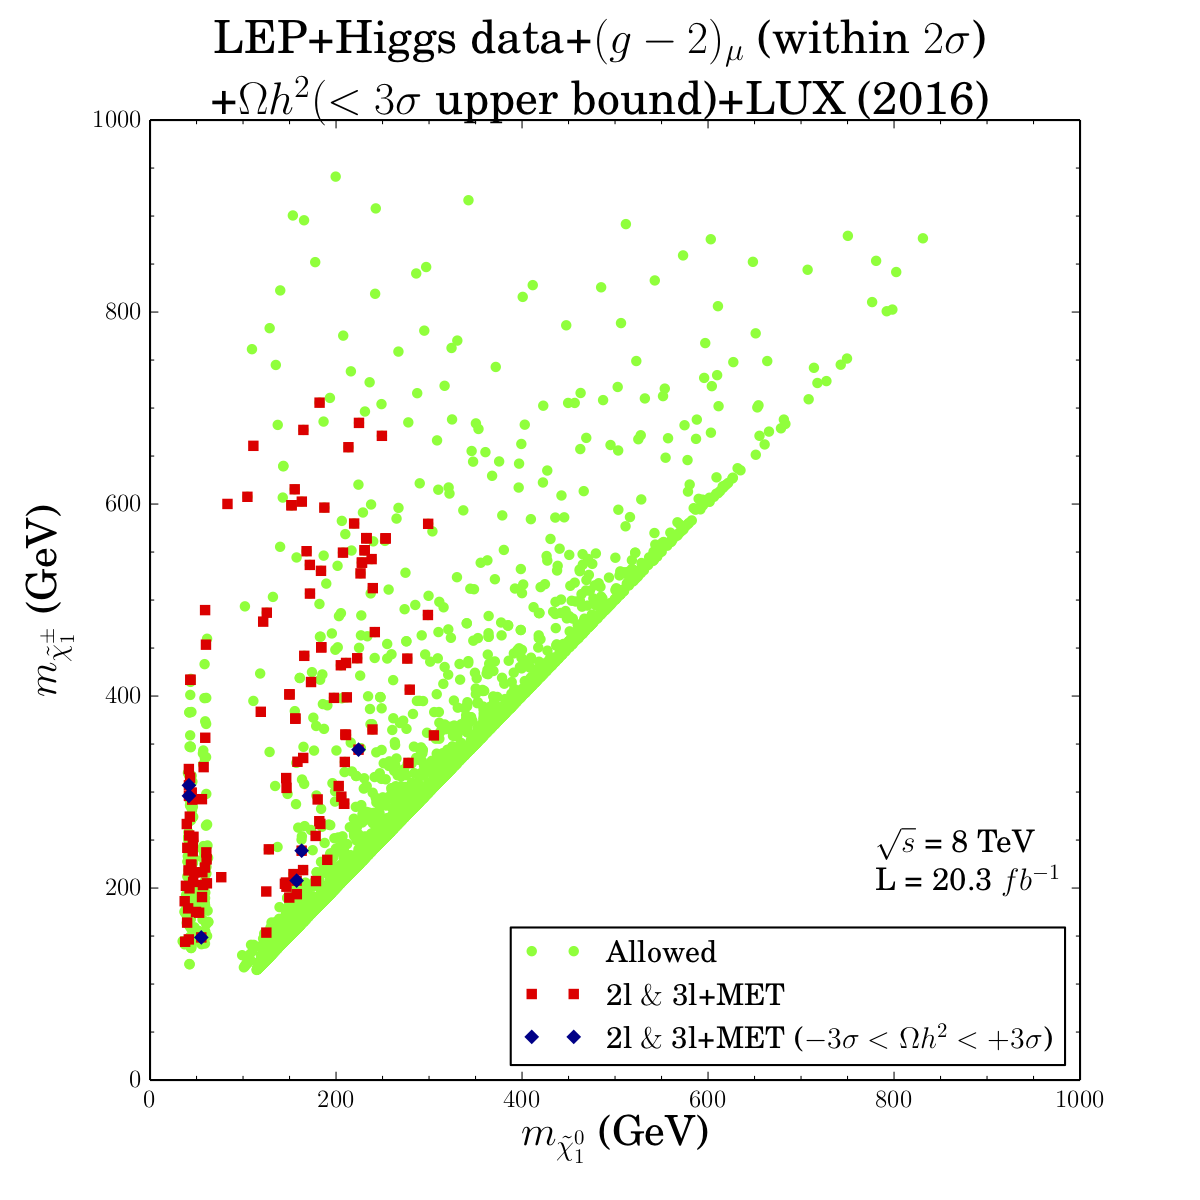
\includegraphics[scale=0.5]{figures/plot8TeV.png}
\captionof{figure}[Exclusion limits from $2\ell+\slashed{E}_T$ \& $3\ell+\slashed{E}_T$ events at $\sqrt{s}=8$ TeV LHC.]{Exclusion limits in the $m_{\tilde{\chi}^{\pm}_1} - m_{\tilde{\chi}^{0}_1}$ plane from LHC Run-I at $\sqrt{s}=8$ TeV from combined dilepton and trilepton events. All samples in the plot satisy LEP and Higgs constraints, $\Delta a_{\mu}$ within $2\sigma$ and the $3\sigma$ upper bound on the relic density as well as the LUX 2016 spin-independent cross-section 95\% C.L. exclusion limits. We sort the excluded $2\ell+\slashed{E}_T$ \& $3\ell+\slashed{E}_T$ samples into $\Omega h^2<+3\sigma$ (red squares) and $-3\sigma <\Omega h^2<+3\sigma$ (blue diamonds) where $\Omega h^2 \equiv \Omega_{DM} h^2 - \Omega_{Planck} h^2$.}
\label{fig:8Tevplot}
\end{center}

In Figure \ref{fig:8Tevplot}, we recast the exclusion limits coming from the LHC 8-TeV dilepton and trilepton searches, shown in the $m_{\tilde{\chi}^{\pm}_1} - m_{\tilde{\chi}^{0}_1}$ plane. All the samples present satisfy $\Delta a_{\mu}$ within $2\sigma$ as well as the LEP, Higgs and other collider constraints. They also satisfy the $3\sigma$ upper bound on the DM relic density and direct detection limits from LUX 2016. We further classify these into the dilepton and trilepton excluded points (blue diamonds), and a subset of these that satisfy both the upper and lower bound on the relic density (red squares). There is a portion of samples that can be excluded by the 8 TeV limits, namely for $\tilde{\chi}^{0}_1<300$ GeV and $\tilde{\chi}^{\pm}_1<710$ GeV. There is a significant number of samples that are not excluded lying around the region where $\tilde{\chi}^{\pm}_1$ and $\tilde{\chi}^{0}_1$ are almost degenerate. These are wino or Higgsino-like neutralino candidates. Scenarios like these are usually referred to as \textit{compressed spectra} since there is a small mass difference, $\Delta m$, between the LSP and the NLSP \cite{RN186}. Typically the soft decay products are difficult to access at the LHC, but can be probed using monojet-like signals to boost the initial state pair and enhance the missing $E_T$ of the final state. It has also been suggested in the Higgsino case to search for soft dileptons complementary to the monojet signal to boost the signal-to-background ratio rather than monojets alone which suffer from large SM background \cite{RN902,RN901,RN900}. Similarly, the small electroweak production rate can be studied in the context of Vector Boson Fusion (\acrshort{vbf}) production at LHC \cite{RN644}. The strategy for these analyses is to search for two forward opposite-hemisphere jets with large dijet invariant mass. Such analyses have been investigated in the context of the HL-LHC \cite{RN186,RN309,RN187,RN188,RN189,RN190,RN191}.
  
However, when the bino component of $\tilde{\chi}^0_2$ becomes dominant, the cross-section from $\tilde{\chi}^{\pm}_1 \tilde{\chi}^0_2$ becomes suppressed. In this case we find that the dilepton searches may become complimentary to the trilepton channel. The factor in determining this is the neutralino-leptonic branching fraction which can be quite sensitive to the configuration of the parameter space. We identify a number of cases:
\begin{enumerate}[label=(\alph*)]
\item When the slepton is on shell, the chargino two-body decay dominates with the leptonic branching fraction given by $\mathcal{B}(\tilde{\chi}^{\pm}_1 \rightarrow \nu_{\ell} \tilde{\ell}^{\pm} (\rightarrow \tilde{\chi}^0_1 \ell^{\pm}))_{\text{max}}=2/3$.
\item When the sneutrino is on-	shell and lighter than the corresponding slepton, the dominant decay mode will be $\tilde{\chi}^0_2 \rightarrow \nu_{\ell} \tilde{\nu_{\ell}}$ with the neutralino leptonic branching fraction suppressed.
\item When the sleptons and sneutrinos are heavy, the decay paths of $\tilde{\chi}^{\pm}_1$ and $\tilde{\chi}^0_2$ are dominated by $W$ and $Z$ decays, respectively. The branching fractions are given by $\mathcal{B}(\tilde{\chi}^{\pm}_1 \rightarrow \tilde{\chi}^0_1 W^{\pm} (\rightarrow \ell^{\pm} \nu_{\ell})) \simeq 2/9$ and $\mathcal{B}(\tilde{\chi}^0_2 \rightarrow \tilde{\chi}^0_1 Z (\rightarrow \ell^{\pm} \ell^{\mp})) \sim 6\%$, respectively. Otherwise if the decay path $\tilde{\chi}^0_1 \rightarrow h \tilde{\chi}^0_1$ is kinematically accessible, then the trilepton exclusion limits can be weakened  in this way.
\end{enumerate}

\section{Prospects for searches at a 100 TeV collider}

The frontier of particle physics hinges on the ability to resolve smaller and smaller distances (higher and higher energy scales) at colliders in order to probe fundamental new physics. In recent years, there have been proposals for a 100 TeV $pp$ collider that could potentially probe an order of magnitude energy scale higher than the LHC \cite{RN619} with promising prospects for detection of charged and neutral SUSY states \cite{RN194,RN195}. The integrated luminosity of such a machine may be as high as 3 ab$^{-1}$, the same as the target luminosity for the \acrshort{hllhc} upgrade, as we will use in this study.

In this section, we study the potential for a 100 TeV $pp$ collider to explain $\Delta a_{\mu}$ and the previous direct search constraints as well as those from DM relic density and LUX 2016. We extrapolate the allowed sample results from the 8 TeV search in the previous section using the most sensitive signal region. In this way, we simply rescale the signal $(S)$ and background $(B)$ events by the following ratio using the corresponding production cross-sections:
\begin{equation}
N^{100\,\text{TeV}}/N^{8\,\text{TeV}}=(\sigma^{100\,\text{TeV}}/\sigma^{8\,\text{TeV}})(\mathcal{L}^{100\,\text{TeV}}/\mathcal{L}^{8\,\text{TeV}}),
\end{equation}
where we have used the luminosities $\mathcal{L}^{8\,\text{TeV}}=20.3\,\text{fb}^{-1}$ and $\mathcal{L}^{100\,\text{TeV}}=3000\,\text{fb}^{-1}$. We consider such a treatment a preliminary theoretical estimate. Optimization of this strategy could be performed once the details of the collider environment become known. The expected signal exclusion criteria for the most sensitive signal region is taken as
\begin{equation}
\frac{S}{\sqrt{B+(\beta_{sys.}B)^2}} \geq 2 \qquad \text{[Excluded]},
\end{equation}
where the dimensionless factor $\beta_{sys.}$ parameterizes the systematic uncertainties. Figure \ref{fig:100Tevplot} shows the expected exclusion limits, where we can see that for $\beta_{sys.}=0.1$ we can probe a number of samples within $\tilde{\chi}^0_1 < 530$ GeV and $\tilde{\chi}^{\pm}_1 < 940$ GeV. This extends to $\tilde{\chi}^0_1 < 710$ GeV and $\tilde{\chi}^{\pm}_1 < 940$ GeV in the case where $\beta_{sys.}=0$.

We note that regions satisfying the relic density within the $3\sigma$ (upper and lower) range, through resonant annihilation in the `blind spot' region can now be searched for through the associated production process $\tilde{\chi}^0_2 \tilde{\chi}^+_1$ at the 100 TeV $pp$ collider. However, there are still samples outside the reach of future searches for trilepton events, corresponding to Higgsino/wino-like LSPs in the compressed mass spectrum region or bino-like LSPs that co-annihilate with the sleptons. The former may be probed through the monojet(-like) analysis at a future 100 TeV $pp$ collider, as explored in \cite{RN196}.

\begin{center}
	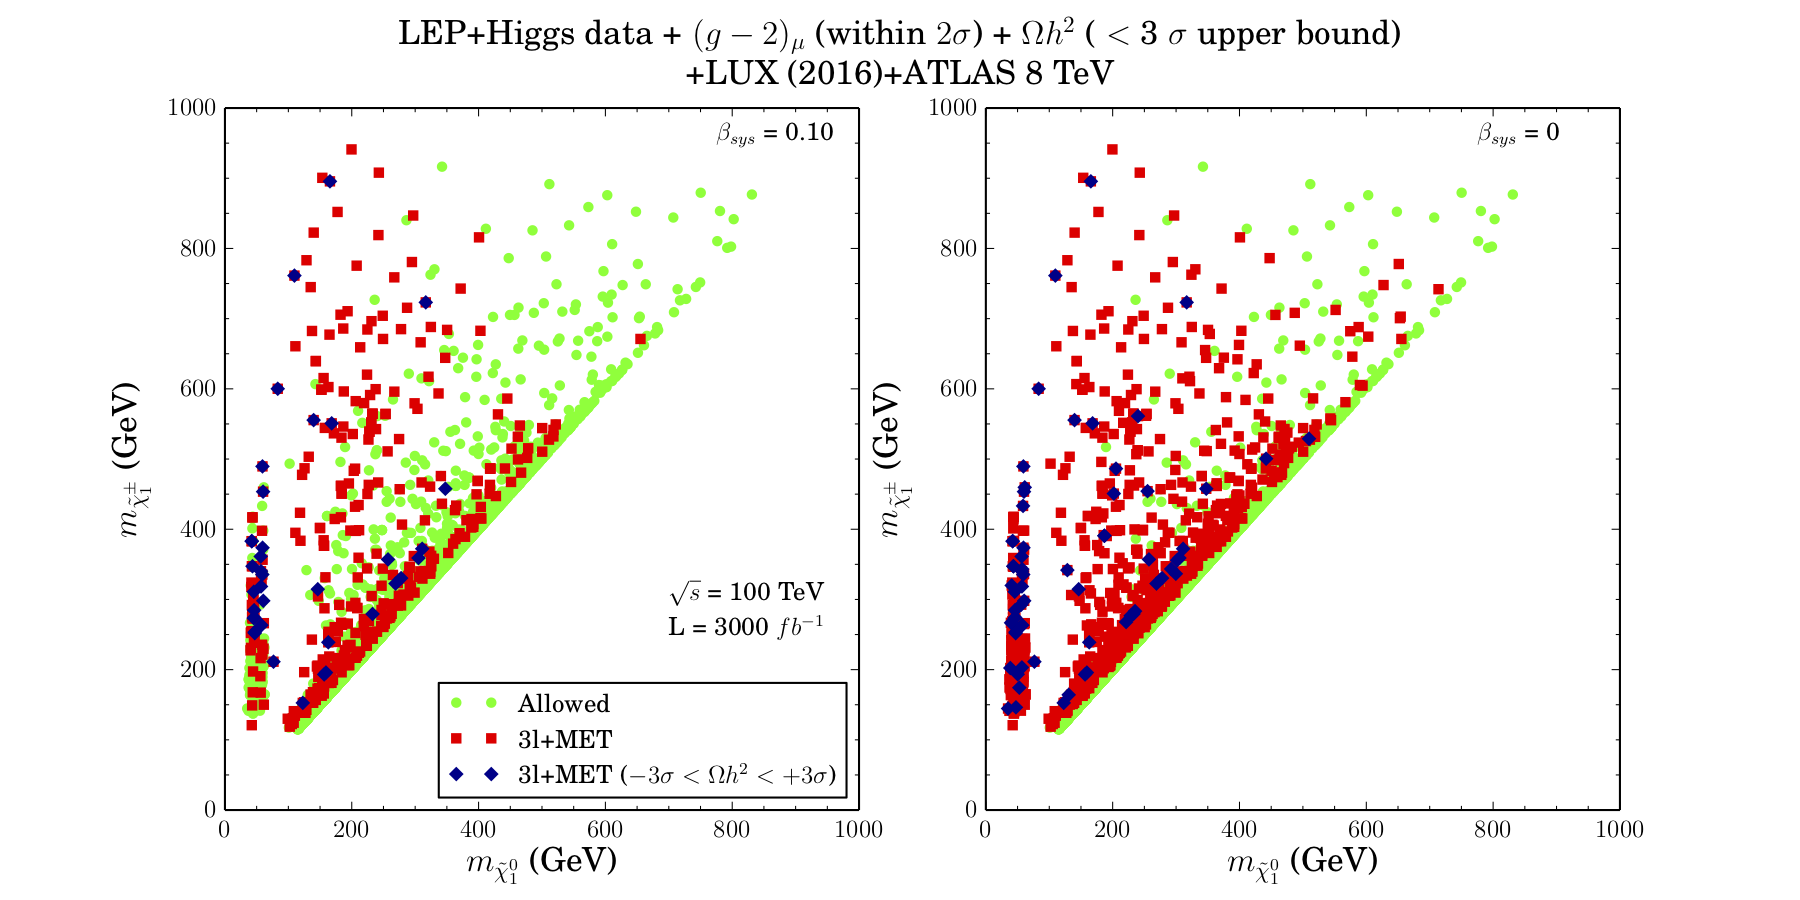
\includegraphics[scale=0.5]{figures/plot100TeV.png}
	\captionof{figure}[Exclusion limits from $2\ell+\slashed{E}_T$ \& $3\ell+\slashed{E}_T$ events at $\sqrt{s}=100$ TeV.]{Same as for Figure \ref{fig:8Tevplot}, but for $\sqrt{s}=100$ TeV and 3000 fb$^{-1}$ of data. Excluded $2\ell+\slashed{E}_T$ \& $3\ell+\slashed{E}_T$ samples are shown for the ranges $\Omega h^2<+3\sigma$ (red squares) and $-3\sigma <\Omega h^2<+3\sigma$ (blue diamonds) where $\Omega h^2 \equiv \Omega_{DM} h^2 - \Omega_{Planck} h^2$. The two figures correspond to $\beta_{sys.}=0.1$ and $\beta_{sys.}=0$, respectively.}
	\label{fig:100Tevplot}
\end{center}

\section{Concluding remarks}

This chapter has combined results from current and future $pp$ coliider and dark matter direct detection experiments to produce limits on the spectrum of electroweak sparticles that satisfy the anomalous magnetic moment of the muon, or $(g-2)_{\mu}$, in the MSSM. With all relevant constraints from Higgs and SUSY searches at LEP and LHC, measurements of the dark matter relic density from Planck and the PANDAX-II/LUX-2016 direct detection experiments, parts of the MSSM parameter space satisfying the $(g-2)_{\mu}$ can be significantly excluded. These limits could be further improved using the recent XENON-1T \cite{RN606,RN770} dark matter constraints and monojet searches \cite{RN196} at the LHC, especially for regions where the mass difference between the LSP and NLSP is small. In a broader context, our naive estimates in Figure \ref{fig:100Tevplot} give further motivation towards direct SUSY searches that shed light on low-energy observables like the $(g-2)_{\mu}$, and furthermore the development of next-generation colliders. It could be argued from these results that after the full run of next generation $pp$ colliders, one could finally close the lid on the simplest versions of supersymmetry satisfying the $(g-2)_{\mu}$ that simultaneously explain all (or part of) the dark matter abundance in the universe.

To close this chapter, we would also like to stress that despite the microscopic properties of the dark matter, the abundance significantly depends on its cosmological evolution of the early universe. More specifically, particular regions of excluded parameter space (i.e. predominantly bino-like LSPs) can actually become consistent with observation through depopulation mechanisms of cosmological origin, which are described in more detail in chapter \ref{chap:wimpdecay}.
